\section{課題の設定と結果}
\begin{frame}{課題の設定と結果}
    先行研究の結果を利用して先手の勝率を可視化して観察した。
    また、観察結果からみられた特徴を数学的に証明することを試みた。
\end{frame}

\begin{frame}{課題の設定と結果}
    先手の勝率の可視化は次の2つの方法に分けて行った。
    \begin{itemize}
        \item ランダムに手を打つプレイヤーのシミュレーションをプログラムで組んで、その時の先手の勝率を可視化
        \item 3行の盤面に固定して、モデル化で提示した再帰式から計算して、その結果をグラフに可視化
    \end{itemize}
\end{frame}

\begin{frame}{課題の設定と結果}
    \begin{figure}
        \centering
        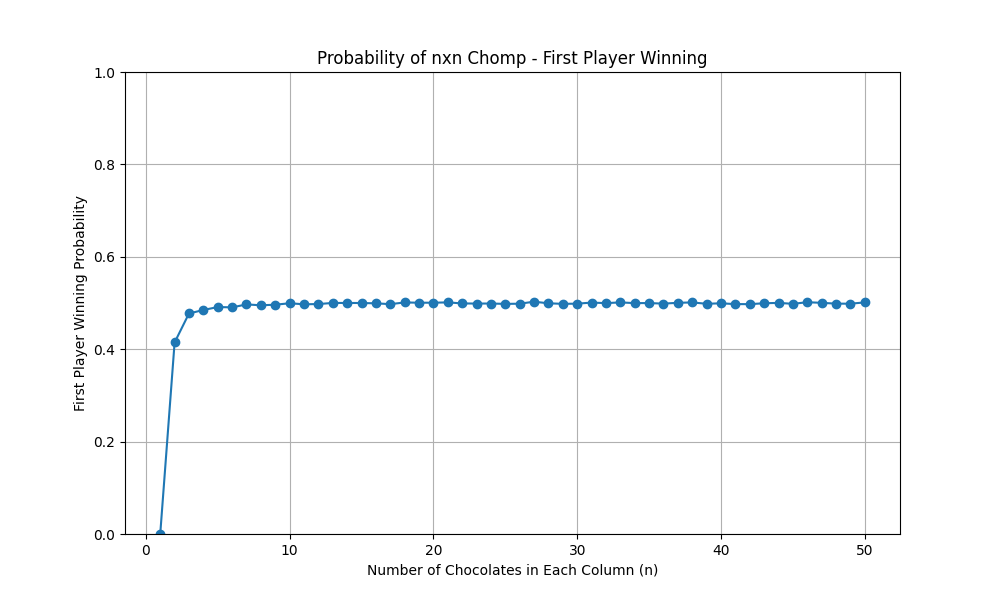
\includegraphics[width=0.6\columnwidth]{research/figures/visualize_simulated_prob.png}
        \caption{シミュレーションの可視化}
    \end{figure}
\end{frame}

\begin{frame}{課題の設定と結果}
    \begin{figure}
        \centering
        \begin{minipage}[b]{0.49\columnwidth}
            \centering
            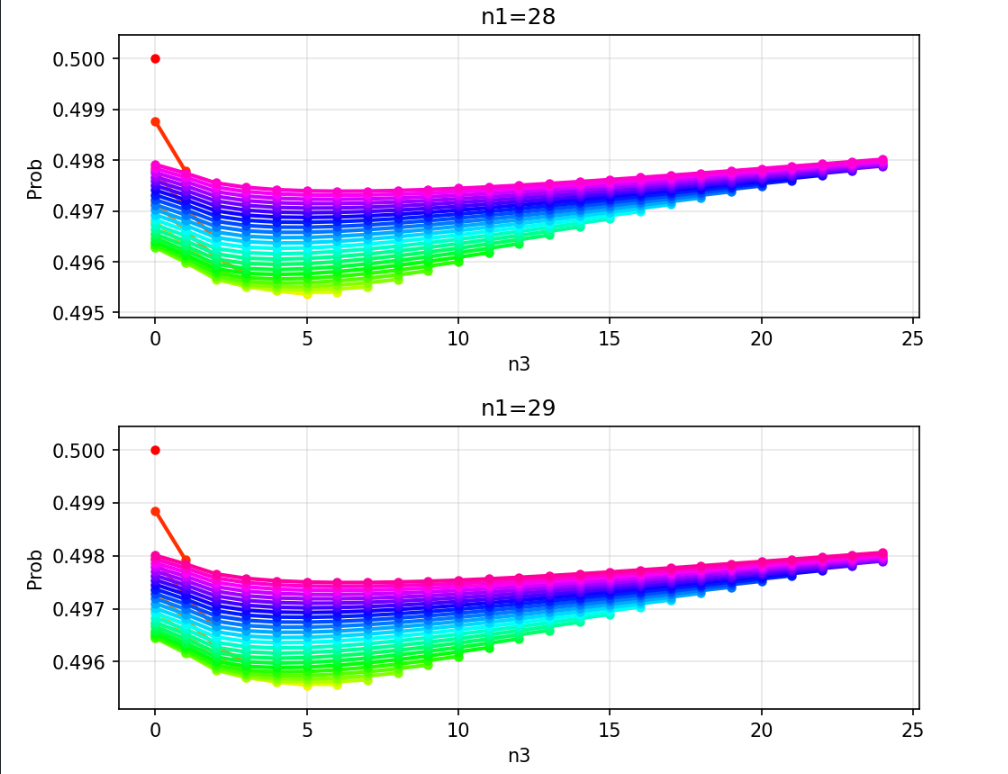
\includegraphics[width=0.9\columnwidth]{research/figures/visualize_prob_overlap_row.png}
        \end{minipage}
        \begin{minipage}[b]{0.49\columnwidth}
            \centering
            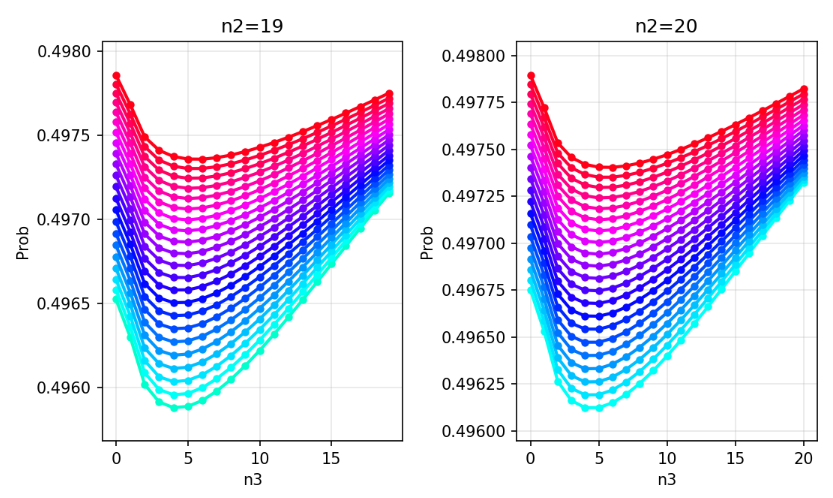
\includegraphics[width=0.9\columnwidth]{research/figures/visualize_prob_overlap_col.png}
        \end{minipage}
        \caption{3行に固定された盤面における先手の勝率の可視化}
    \end{figure}
\end{frame}

\begin{frame}{課題の設定と結果}
    可視化から、以下のことを考えた。
    \begin{itemize}
        \item ある一定のところを超えると確率が単調に増加する
        \item 勝率は(見える範囲では)\(0.5\)を下回っている
    \end{itemize}
\end{frame}

\begin{frame}{課題の設定と結果}
    \begin{block}{盤面の包含関係と確率の単調性についての予想}
        盤面\(B\)と\(B'\)について、2つの盤面の間に\(|B| = |B'| + 1\)という関係があり、かつ\(|B|\)が十分に大きいとき
        \begin{equation}
            P(B) \geq P(B')
        \end{equation}
        という関係がある
    \end{block}
\end{frame}

\begin{frame}{課題の設定とその結果}
    \begin{block}{盤面の包含関係と確率の大小関係についての予想}
        \begin{align}
            P(B) - P(B')    &= \left(1 - \frac{1}{|B|} \sum_{B \rightarrow C} P(C)\right) - \left(1 - \frac{1}{|B'|} \sum_{B' \rightarrow C} P(C)\right) \\
                            &= \sum_{B' \rightarrow C} \left(\frac{1}{|B'|} - \frac{1}{|B|}\right) P(C) - \frac{P(B')}{|B|} \\
                            &= \sum_{B' \rightarrow C} \frac{1}{|B||B'|} P(C) - \frac{1}{|B|} \left(1 - \frac{1}{|B'|}\sum_{B' \rightarrow C} P(C)\right) \\
                            &= \frac{2}{|B||B'|} \sum_{B' \rightarrow C} P(C) - \frac{1}{|B|}
        \end{align}
    \end{block}
\end{frame}